\documentclass{article} % For LaTeX2e

\usepackage{appendix}
\usepackage{intern}
% Remove times package as it conflicts with other font packages
% \usepackage{times}  

% Use Computer Modern (classic LaTeX font) instead of Palatino
% \usepackage{mathpazo}
\usepackage{microtype}   % Keep microtype for better typography
\linespread{1.10}        % Slightly increase line spacing for better readability

% Optional math commands from https://github.com/goodfeli/dlbook_notation.
%%%%% NEW MATH DEFINITIONS %%%%%

\usepackage{amsmath,amsfonts,bm}

% Mark sections of captions for referring to divisions of figures
\newcommand{\figleft}{{\em (Left)}}
\newcommand{\figcenter}{{\em (Center)}}
\newcommand{\figright}{{\em (Right)}}
\newcommand{\figtop}{{\em (Top)}}
\newcommand{\figbottom}{{\em (Bottom)}}
\newcommand{\captiona}{{\em (a)}}
\newcommand{\captionb}{{\em (b)}}
\newcommand{\captionc}{{\em (c)}}
\newcommand{\captiond}{{\em (d)}}

% Highlight a newly defined term
\newcommand{\newterm}[1]{{\bf #1}}


% Figure reference, lower-case.
\def\figref#1{figure~\ref{#1}}
% Figure reference, capital. For start of sentence
\def\Figref#1{Figure~\ref{#1}}
\def\twofigref#1#2{figures \ref{#1} and \ref{#2}}
\def\quadfigref#1#2#3#4{figures \ref{#1}, \ref{#2}, \ref{#3} and \ref{#4}}
% Section reference, lower-case.
\def\secref#1{section~\ref{#1}}
% Section reference, capital.
\def\Secref#1{Section~\ref{#1}}
% Reference to two sections.
\def\twosecrefs#1#2{sections \ref{#1} and \ref{#2}}
% Reference to three sections.
\def\secrefs#1#2#3{sections \ref{#1}, \ref{#2} and \ref{#3}}
% Reference to an equation, lower-case.
\def\eqref#1{equation~\ref{#1}}
% Reference to an equation, upper case
\def\Eqref#1{Equation~\ref{#1}}
% A raw reference to an equation---avoid using if possible
\def\plaineqref#1{\ref{#1}}
% Reference to a chapter, lower-case.
\def\chapref#1{chapter~\ref{#1}}
% Reference to an equation, upper case.
\def\Chapref#1{Chapter~\ref{#1}}
% Reference to a range of chapters
\def\rangechapref#1#2{chapters\ref{#1}--\ref{#2}}
% Reference to an algorithm, lower-case.
\def\algref#1{algorithm~\ref{#1}}
% Reference to an algorithm, upper case.
\def\Algref#1{Algorithm~\ref{#1}}
\def\twoalgref#1#2{algorithms \ref{#1} and \ref{#2}}
\def\Twoalgref#1#2{Algorithms \ref{#1} and \ref{#2}}
% Reference to a part, lower case
\def\partref#1{part~\ref{#1}}
% Reference to a part, upper case
\def\Partref#1{Part~\ref{#1}}
\def\twopartref#1#2{parts \ref{#1} and \ref{#2}}

\def\ceil#1{\lceil #1 \rceil}
\def\floor#1{\lfloor #1 \rfloor}
\def\1{\bm{1}}
\newcommand{\train}{\mathcal{D}}
\newcommand{\valid}{\mathcal{D_{\mathrm{valid}}}}
\newcommand{\test}{\mathcal{D_{\mathrm{test}}}}

\def\eps{{\epsilon}}


% Random variables
\def\reta{{\textnormal{$\eta$}}}
\def\ra{{\textnormal{a}}}
\def\rb{{\textnormal{b}}}
\def\rc{{\textnormal{c}}}
\def\rd{{\textnormal{d}}}
\def\re{{\textnormal{e}}}
\def\rf{{\textnormal{f}}}
\def\rg{{\textnormal{g}}}
\def\rh{{\textnormal{h}}}
\def\ri{{\textnormal{i}}}
\def\rj{{\textnormal{j}}}
\def\rk{{\textnormal{k}}}
\def\rl{{\textnormal{l}}}
% rm is already a command, just don't name any random variables m
\def\rn{{\textnormal{n}}}
\def\ro{{\textnormal{o}}}
\def\rp{{\textnormal{p}}}
\def\rq{{\textnormal{q}}}
\def\rr{{\textnormal{r}}}
\def\rs{{\textnormal{s}}}
\def\rt{{\textnormal{t}}}
\def\ru{{\textnormal{u}}}
\def\rv{{\textnormal{v}}}
\def\rw{{\textnormal{w}}}
\def\rx{{\textnormal{x}}}
\def\ry{{\textnormal{y}}}
\def\rz{{\textnormal{z}}}

% Random vectors
\def\rvepsilon{{\mathbf{\epsilon}}}
\def\rvtheta{{\mathbf{\theta}}}
\def\rva{{\mathbf{a}}}
\def\rvb{{\mathbf{b}}}
\def\rvc{{\mathbf{c}}}
\def\rvd{{\mathbf{d}}}
\def\rve{{\mathbf{e}}}
\def\rvf{{\mathbf{f}}}
\def\rvg{{\mathbf{g}}}
\def\rvh{{\mathbf{h}}}
\def\rvu{{\mathbf{i}}}
\def\rvj{{\mathbf{j}}}
\def\rvk{{\mathbf{k}}}
\def\rvl{{\mathbf{l}}}
\def\rvm{{\mathbf{m}}}
\def\rvn{{\mathbf{n}}}
\def\rvo{{\mathbf{o}}}
\def\rvp{{\mathbf{p}}}
\def\rvq{{\mathbf{q}}}
\def\rvr{{\mathbf{r}}}
\def\rvs{{\mathbf{s}}}
\def\rvt{{\mathbf{t}}}
\def\rvu{{\mathbf{u}}}
\def\rvv{{\mathbf{v}}}
\def\rvw{{\mathbf{w}}}
\def\rvx{{\mathbf{x}}}
\def\rvy{{\mathbf{y}}}
\def\rvz{{\mathbf{z}}}

% Elements of random vectors
\def\erva{{\textnormal{a}}}
\def\ervb{{\textnormal{b}}}
\def\ervc{{\textnormal{c}}}
\def\ervd{{\textnormal{d}}}
\def\erve{{\textnormal{e}}}
\def\ervf{{\textnormal{f}}}
\def\ervg{{\textnormal{g}}}
\def\ervh{{\textnormal{h}}}
\def\ervi{{\textnormal{i}}}
\def\ervj{{\textnormal{j}}}
\def\ervk{{\textnormal{k}}}
\def\ervl{{\textnormal{l}}}
\def\ervm{{\textnormal{m}}}
\def\ervn{{\textnormal{n}}}
\def\ervo{{\textnormal{o}}}
\def\ervp{{\textnormal{p}}}
\def\ervq{{\textnormal{q}}}
\def\ervr{{\textnormal{r}}}
\def\ervs{{\textnormal{s}}}
\def\ervt{{\textnormal{t}}}
\def\ervu{{\textnormal{u}}}
\def\ervv{{\textnormal{v}}}
\def\ervw{{\textnormal{w}}}
\def\ervx{{\textnormal{x}}}
\def\ervy{{\textnormal{y}}}
\def\ervz{{\textnormal{z}}}

% Random matrices
\def\rmA{{\mathbf{A}}}
\def\rmB{{\mathbf{B}}}
\def\rmC{{\mathbf{C}}}
\def\rmD{{\mathbf{D}}}
\def\rmE{{\mathbf{E}}}
\def\rmF{{\mathbf{F}}}
\def\rmG{{\mathbf{G}}}
\def\rmH{{\mathbf{H}}}
\def\rmI{{\mathbf{I}}}
\def\rmJ{{\mathbf{J}}}
\def\rmK{{\mathbf{K}}}
\def\rmL{{\mathbf{L}}}
\def\rmM{{\mathbf{M}}}
\def\rmN{{\mathbf{N}}}
\def\rmO{{\mathbf{O}}}
\def\rmP{{\mathbf{P}}}
\def\rmQ{{\mathbf{Q}}}
\def\rmR{{\mathbf{R}}}
\def\rmS{{\mathbf{S}}}
\def\rmT{{\mathbf{T}}}
\def\rmU{{\mathbf{U}}}
\def\rmV{{\mathbf{V}}}
\def\rmW{{\mathbf{W}}}
\def\rmX{{\mathbf{X}}}
\def\rmY{{\mathbf{Y}}}
\def\rmZ{{\mathbf{Z}}}

% Elements of random matrices
\def\ermA{{\textnormal{A}}}
\def\ermB{{\textnormal{B}}}
\def\ermC{{\textnormal{C}}}
\def\ermD{{\textnormal{D}}}
\def\ermE{{\textnormal{E}}}
\def\ermF{{\textnormal{F}}}
\def\ermG{{\textnormal{G}}}
\def\ermH{{\textnormal{H}}}
\def\ermI{{\textnormal{I}}}
\def\ermJ{{\textnormal{J}}}
\def\ermK{{\textnormal{K}}}
\def\ermL{{\textnormal{L}}}
\def\ermM{{\textnormal{M}}}
\def\ermN{{\textnormal{N}}}
\def\ermO{{\textnormal{O}}}
\def\ermP{{\textnormal{P}}}
\def\ermQ{{\textnormal{Q}}}
\def\ermR{{\textnormal{R}}}
\def\ermS{{\textnormal{S}}}
\def\ermT{{\textnormal{T}}}
\def\ermU{{\textnormal{U}}}
\def\ermV{{\textnormal{V}}}
\def\ermW{{\textnormal{W}}}
\def\ermX{{\textnormal{X}}}
\def\ermY{{\textnormal{Y}}}
\def\ermZ{{\textnormal{Z}}}

% Vectors
\def\vzero{{\bm{0}}}
\def\vone{{\bm{1}}}
\def\vmu{{\bm{\mu}}}
\def\vtheta{{\bm{\theta}}}
\def\va{{\bm{a}}}
\def\vb{{\bm{b}}}
\def\vc{{\bm{c}}}
\def\vd{{\bm{d}}}
\def\ve{{\bm{e}}}
\def\vf{{\bm{f}}}
\def\vg{{\bm{g}}}
\def\vh{{\bm{h}}}
\def\vi{{\bm{i}}}
\def\vj{{\bm{j}}}
\def\vk{{\bm{k}}}
\def\vl{{\bm{l}}}
\def\vm{{\bm{m}}}
\def\vn{{\bm{n}}}
\def\vo{{\bm{o}}}
\def\vp{{\bm{p}}}
\def\vq{{\bm{q}}}
\def\vr{{\bm{r}}}
\def\vs{{\bm{s}}}
\def\vt{{\bm{t}}}
\def\vu{{\bm{u}}}
\def\vv{{\bm{v}}}
\def\vw{{\bm{w}}}
\def\vx{{\bm{x}}}
\def\vy{{\bm{y}}}
\def\vz{{\bm{z}}}

% Elements of vectors
\def\evalpha{{\alpha}}
\def\evbeta{{\beta}}
\def\evepsilon{{\epsilon}}
\def\evlambda{{\lambda}}
\def\evomega{{\omega}}
\def\evmu{{\mu}}
\def\evpsi{{\psi}}
\def\evsigma{{\sigma}}
\def\evtheta{{\theta}}
\def\eva{{a}}
\def\evb{{b}}
\def\evc{{c}}
\def\evd{{d}}
\def\eve{{e}}
\def\evf{{f}}
\def\evg{{g}}
\def\evh{{h}}
\def\evi{{i}}
\def\evj{{j}}
\def\evk{{k}}
\def\evl{{l}}
\def\evm{{m}}
\def\evn{{n}}
\def\evo{{o}}
\def\evp{{p}}
\def\evq{{q}}
\def\evr{{r}}
\def\evs{{s}}
\def\evt{{t}}
\def\evu{{u}}
\def\evv{{v}}
\def\evw{{w}}
\def\evx{{x}}
\def\evy{{y}}
\def\evz{{z}}

% Matrix
\def\mA{{\bm{A}}}
\def\mB{{\bm{B}}}
\def\mC{{\bm{C}}}
\def\mD{{\bm{D}}}
\def\mE{{\bm{E}}}
\def\mF{{\bm{F}}}
\def\mG{{\bm{G}}}
\def\mH{{\bm{H}}}
\def\mI{{\bm{I}}}
\def\mJ{{\bm{J}}}
\def\mK{{\bm{K}}}
\def\mL{{\bm{L}}}
\def\mM{{\bm{M}}}
\def\mN{{\bm{N}}}
\def\mO{{\bm{O}}}
\def\mP{{\bm{P}}}
\def\mQ{{\bm{Q}}}
\def\mR{{\bm{R}}}
\def\mS{{\bm{S}}}
\def\mT{{\bm{T}}}
\def\mU{{\bm{U}}}
\def\mV{{\bm{V}}}
\def\mW{{\bm{W}}}
\def\mX{{\bm{X}}}
\def\mY{{\bm{Y}}}
\def\mZ{{\bm{Z}}}
\def\mBeta{{\bm{\beta}}}
\def\mPhi{{\bm{\Phi}}}
\def\mLambda{{\bm{\Lambda}}}
\def\mSigma{{\bm{\Sigma}}}

% Tensor
\DeclareMathAlphabet{\mathsfit}{\encodingdefault}{\sfdefault}{m}{sl}
\SetMathAlphabet{\mathsfit}{bold}{\encodingdefault}{\sfdefault}{bx}{n}
\newcommand{\tens}[1]{\bm{\mathsfit{#1}}}
\def\tA{{\tens{A}}}
\def\tB{{\tens{B}}}
\def\tC{{\tens{C}}}
\def\tD{{\tens{D}}}
\def\tE{{\tens{E}}}
\def\tF{{\tens{F}}}
\def\tG{{\tens{G}}}
\def\tH{{\tens{H}}}
\def\tI{{\tens{I}}}
\def\tJ{{\tens{J}}}
\def\tK{{\tens{K}}}
\def\tL{{\tens{L}}}
\def\tM{{\tens{M}}}
\def\tN{{\tens{N}}}
\def\tO{{\tens{O}}}
\def\tP{{\tens{P}}}
\def\tQ{{\tens{Q}}}
\def\tR{{\tens{R}}}
\def\tS{{\tens{S}}}
\def\tT{{\tens{T}}}
\def\tU{{\tens{U}}}
\def\tV{{\tens{V}}}
\def\tW{{\tens{W}}}
\def\tX{{\tens{X}}}
\def\tY{{\tens{Y}}}
\def\tZ{{\tens{Z}}}


% Graph
\def\gA{{\mathcal{A}}}
\def\gB{{\mathcal{B}}}
\def\gC{{\mathcal{C}}}
\def\gD{{\mathcal{D}}}
\def\gE{{\mathcal{E}}}
\def\gF{{\mathcal{F}}}
\def\gG{{\mathcal{G}}}
\def\gH{{\mathcal{H}}}
\def\gI{{\mathcal{I}}}
\def\gJ{{\mathcal{J}}}
\def\gK{{\mathcal{K}}}
\def\gL{{\mathcal{L}}}
\def\gM{{\mathcal{M}}}
\def\gN{{\mathcal{N}}}
\def\gO{{\mathcal{O}}}
\def\gP{{\mathcal{P}}}
\def\gQ{{\mathcal{Q}}}
\def\gR{{\mathcal{R}}}
\def\gS{{\mathcal{S}}}
\def\gT{{\mathcal{T}}}
\def\gU{{\mathcal{U}}}
\def\gV{{\mathcal{V}}}
\def\gW{{\mathcal{W}}}
\def\gX{{\mathcal{X}}}
\def\gY{{\mathcal{Y}}}
\def\gZ{{\mathcal{Z}}}

% Sets
\def\sA{{\mathbb{A}}}
\def\sB{{\mathbb{B}}}
\def\sC{{\mathbb{C}}}
\def\sD{{\mathbb{D}}}
% Don't use a set called E, because this would be the same as our symbol
% for expectation.
\def\sF{{\mathbb{F}}}
\def\sG{{\mathbb{G}}}
\def\sH{{\mathbb{H}}}
\def\sI{{\mathbb{I}}}
\def\sJ{{\mathbb{J}}}
\def\sK{{\mathbb{K}}}
\def\sL{{\mathbb{L}}}
\def\sM{{\mathbb{M}}}
\def\sN{{\mathbb{N}}}
\def\sO{{\mathbb{O}}}
\def\sP{{\mathbb{P}}}
\def\sQ{{\mathbb{Q}}}
\def\sR{{\mathbb{R}}}
\def\sS{{\mathbb{S}}}
\def\sT{{\mathbb{T}}}
\def\sU{{\mathbb{U}}}
\def\sV{{\mathbb{V}}}
\def\sW{{\mathbb{W}}}
\def\sX{{\mathbb{X}}}
\def\sY{{\mathbb{Y}}}
\def\sZ{{\mathbb{Z}}}

% Entries of a matrix
\def\emLambda{{\Lambda}}
\def\emA{{A}}
\def\emB{{B}}
\def\emC{{C}}
\def\emD{{D}}
\def\emE{{E}}
\def\emF{{F}}
\def\emG{{G}}
\def\emH{{H}}
\def\emI{{I}}
\def\emJ{{J}}
\def\emK{{K}}
\def\emL{{L}}
\def\emM{{M}}
\def\emN{{N}}
\def\emO{{O}}
\def\emP{{P}}
\def\emQ{{Q}}
\def\emR{{R}}
\def\emS{{S}}
\def\emT{{T}}
\def\emU{{U}}
\def\emV{{V}}
\def\emW{{W}}
\def\emX{{X}}
\def\emY{{Y}}
\def\emZ{{Z}}
\def\emSigma{{\Sigma}}

% entries of a tensor
% Same font as tensor, without \bm wrapper
\newcommand{\etens}[1]{\mathsfit{#1}}
\def\etLambda{{\etens{\Lambda}}}
\def\etA{{\etens{A}}}
\def\etB{{\etens{B}}}
\def\etC{{\etens{C}}}
\def\etD{{\etens{D}}}
\def\etE{{\etens{E}}}
\def\etF{{\etens{F}}}
\def\etG{{\etens{G}}}
\def\etH{{\etens{H}}}
\def\etI{{\etens{I}}}
\def\etJ{{\etens{J}}}
\def\etK{{\etens{K}}}
\def\etL{{\etens{L}}}
\def\etM{{\etens{M}}}
\def\etN{{\etens{N}}}
\def\etO{{\etens{O}}}
\def\etP{{\etens{P}}}
\def\etQ{{\etens{Q}}}
\def\etR{{\etens{R}}}
\def\etS{{\etens{S}}}
\def\etT{{\etens{T}}}
\def\etU{{\etens{U}}}
\def\etV{{\etens{V}}}
\def\etW{{\etens{W}}}
\def\etX{{\etens{X}}}
\def\etY{{\etens{Y}}}
\def\etZ{{\etens{Z}}}

% The true underlying data generating distribution
\newcommand{\pdata}{p_{\rm{data}}}
% The empirical distribution defined by the training set
\newcommand{\ptrain}{\hat{p}_{\rm{data}}}
\newcommand{\Ptrain}{\hat{P}_{\rm{data}}}
% The model distribution
\newcommand{\pmodel}{p_{\rm{model}}}
\newcommand{\Pmodel}{P_{\rm{model}}}
\newcommand{\ptildemodel}{\tilde{p}_{\rm{model}}}
% Stochastic autoencoder distributions
\newcommand{\pencode}{p_{\rm{encoder}}}
\newcommand{\pdecode}{p_{\rm{decoder}}}
\newcommand{\precons}{p_{\rm{reconstruct}}}

\newcommand{\laplace}{\mathrm{Laplace}} % Laplace distribution

\newcommand{\E}{\mathbb{E}}
\newcommand{\Ls}{\mathcal{L}}
\newcommand{\R}{\mathbb{R}}
\newcommand{\emp}{\tilde{p}}
\newcommand{\lr}{\alpha}
\newcommand{\reg}{\lambda}
\newcommand{\rect}{\mathrm{rectifier}}
\newcommand{\softmax}{\mathrm{softmax}}
\newcommand{\sigmoid}{\sigma}
\newcommand{\softplus}{\zeta}
\newcommand{\KL}{D_{\mathrm{KL}}}
\newcommand{\Var}{\mathrm{Var}}
\newcommand{\standarderror}{\mathrm{SE}}
\newcommand{\Cov}{\mathrm{Cov}}
% Wolfram Mathworld says $L^2$ is for function spaces and $\ell^2$ is for vectors
% But then they seem to use $L^2$ for vectors throughout the site, and so does
% wikipedia.
\newcommand{\normlzero}{L^0}
\newcommand{\normlone}{L^1}
\newcommand{\normltwo}{L^2}
\newcommand{\normlp}{L^p}
\newcommand{\normmax}{L^\infty}

\newcommand{\parents}{Pa} % See usage in notation.tex. Chosen to match Daphne's book.

\DeclareMathOperator*{\argmax}{arg\,max}
\DeclareMathOperator*{\argmin}{arg\,min}

\DeclareMathOperator{\sign}{sign}
\DeclareMathOperator{\Tr}{Tr}
\let\ab\allowbreak


\usepackage{hyperref}
\usepackage{url}
\usepackage{subfigure}
\usepackage{wrapfig}
\usepackage{amsmath,amsthm} % Load amsthm with amsmath
\usepackage{amssymb,amsfonts} %ams symbols after amsthm
\usepackage{enumerate,tikz,graphicx,mathrsfs,eucal,verbatim, bbm}
% \usepackage{enumerate,tikz,graphicx,mathrsfs,eucal,verbatim, bbm, derivative} % Keep derivative here if installed, otherwise remove it.
% \usepackage[ruled,vlined]{algorithm2e}

% Optional: adjust paragraph spacing
\setlength{\parskip}{0.5ex plus 0.3ex minus 0.2ex}

% Optional: adjust margins if needed
\usepackage[margin=1in]{geometry}

\theoremstyle{definition}
\newtheorem{defn}{Definition}[section]

\title{Benchmarking Foundation Models for Robotic Deformable Object Manipulation}

% Authors must not appear in the submitted version. They should be hidden
% as long as the \iclrfinalcopy macro remains commented out below.
% Non-anonymous submissions will be rejected without review.

% \author{Antiquus S.~Hippocampus, Natalia Cerebro \& Amelie P. Amygdale \thanks{ Use footnote for providing further information
% about author (webpage, alternative address)---\emph{not} for acknowledging
% funding agencies.  Funding acknowledgements go at the end of the paper.} \\
% Department of Computer Science\\
% Cranberry-Lemon University\\
% Pittsburgh, PA 15213, USA \\
% \texttt{\{hippo,brain,jen\}@cs.cranberry-lemon.edu} \\
% \And
% Ji Q. Ren \& Yevgeny LeNet \\
% Department of Computational Neuroscience \\
% University of the Witwatersrand \\
% Joburg, South Africa \\
% \texttt{\{robot,net\}@wits.ac.za} \\
% \AND
% Coauthor \\
% Affiliation \\
% Address \\
% \texttt{email}
% }

% The \author macro works with any number of authors. There are two commands
% used to separate the names and addresses of multiple authors: \And and \AND.
%
% Using \And between authors leaves it to \LaTeX{} to determine where to break
% the lines. Using \AND forces a linebreak at that point. So, if \LaTeX{}
% puts 3 of 4 authors names on the first line, and the last on the second
% line, try using \AND instead of \And before the third author name.

\newcommand{\fix}{\marginpar{FIX}}
\newcommand{\new}{\marginpar{NEW}}

\definecolor{orange}{RGB}{252, 130, 62}
\definecolor{red}{RGB}{255, 0, 0}
\definecolor{brown}{RGB}{155, 25, 10}
\definecolor{blue}{RGB}{0, 0,255}
\definecolor{green}{RGB}{78, 196, 164}
\newcommand{\al}{\color{blue}}
\newcommand{\ar}{\color{cyan}}
\newcommand{\ma}{\color{orange}}
\newcommand{\red}{\color{red}}

%\iclrfinalcopy % Uncomment for camera-ready version, but NOT for submission.
\begin{document}


\maketitle


% --- Main ---
\section{Introduction}


Since the publication of RT-1 \cite{RT-1} the robotics research is undergoing a prolific period focused around foundation models. The central promise of this paradigm is the development of generalist policies that aim to achieve general-purpose embodied intelligence, capable of complex interactions within unstructured environments. This shift mirrors advancements in Machine Learning, particularly in Natural Language Processing and Computer Vision, where large pretrained models have demonstrated remarkable success.

\begin{wrapfigure}{r}{0.55\textwidth}
    \centering
    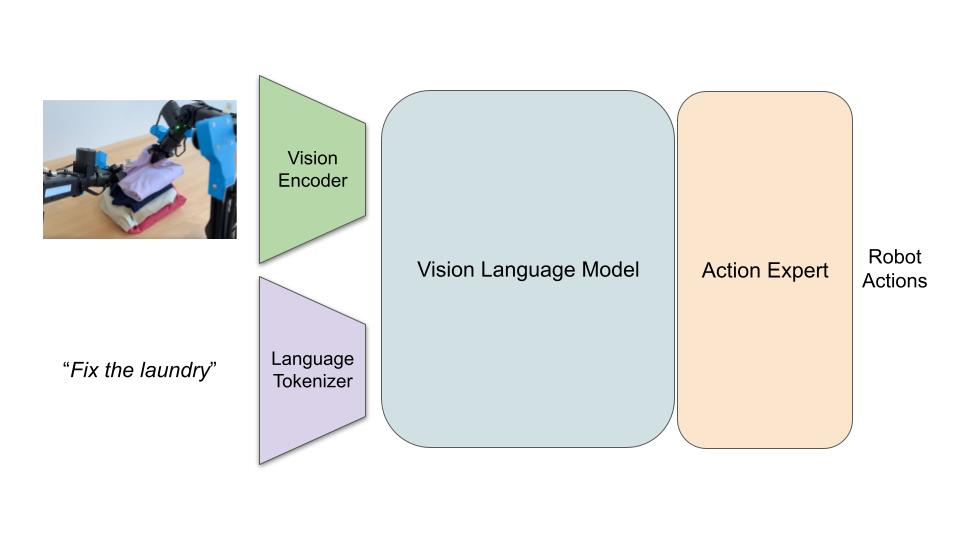
\includegraphics[width=0.55\textwidth]{images/vla.jpg}
    \caption{VLA abstraction}
    \label{fig:mesh}
\end{wrapfigure}

Robotics foundational models, often referred to as Vision-Language-Action (VLA) models, is the name of the policies emerging from this paradigm shift. This nomenclature reflects their modality inputs, vision and language, and outputs, action. Leveraging techniques such as Imitation Learning, Reinforcement Learning, and Self-Supervised Learning, these models have demonstrated remarkable capabilities in dexterous manipulation across multiple tasks, offering a degree of generalization over robot embodiments and environments. A key enabler of this progress is the rise of large-scale pre-training which utilize vast datasets to construct general-purpose representations, applicable across diverse robotic settings, tasks, and embodiments \cite{TransferWelle}.



\section{Goals and Objectives}
Due to their rapid success, the field lacks a standardized benchmarking literature, a critical component for ensuring coherent and equitable expansion. While some work, such as the $\pi_0$ model \cite{pi_zero}, showcase tasks involving deformable object manipulation (e.g., laundry folding), a unified approach for comparing models remains absent. Current efforts often focus on testing single models rather than comparing multiple foundational models to elucidate their differences. This proposal aims to address this gap by developing a Deformable Object Manipulation Benchmarking suite for Robotics Foundation Models, fostering a deeper understanding of their capabilities and limitations. Specifically, we will empirically evaluate how the choices made when building a model (architectural, training recipe, tasks covered, etc.) affect performance on the model capabilities. For example, we will compare the Action Decoder: Diffusion Transformer \cite{Gr00tN1} vs flow matching \cite{pi_zero} vs decoding directly from the pretrained vision language model \cite{OpenVLA}.

\subsection{Overall Goal}

This project aims to deliver:

    \begin{enumerate}
        \item Benchmark suite to evaluate robotics foundational models against deformable object manipulation
        \item Evaluation protocol, applied to the selected policies 
        \item Summarization of the work in a paper
    \end{enumerate}


\subsection{Specific Objectives:}
    \textbf{Literature Review}
        Conduct a comprehensive review, including but not limited to:
        \begin{itemize}
            \item Existing robotics benchmarks, evaluation methodologies, and taxonomies focusing on deformable object manipulation.
            \item Robotics foundational models, emphasizing architectures, training data, and intended capabilities.
        \end{itemize}
    \textbf{Benchmark Design}
        Propose a standardized benchmark suite that integrates and/or extends existing ones and an evaluation protocol. This includes defining clear metrics to provide multidimensional insights of the models' abilities beyond mere performance, such as:
        \begin{itemize}
            \item \textit{Generalization}: Formalize the variations across environments (ex: 1. RPL Laboratory 2. Simulation (GarmentLab, DaXBench, ...), tasks (ex: Cloth Folding, Rope knotting, Sponge ..., Liquid Pouring), and robot embodiments (..., SO-100). (FORMALIZE BETTER?)
            \item \textit{Data efficiency}: Specify how to measure performance across scaling the number of samples the policy consumes: zero-shot, few-shot performance. (FORMALIZE BETTER?)
            \item (Stretch Goal) \textit{Context horizon}: Expand the type of tasks taken into account to quantitatively investigate the horizon each model is able to sustain to solve a task: short-term versus long-term task performance. (FORMALIZE BETTER?)
            \item (Stretch Goal) \textit{Explainable AI}: usage of explainable AI methods such as probing \cite{Probing-VLA} to gain measures of understanding from the internal feature representations of the model. (FORMALIZE BETTER?)
        \end{itemize}
        % \item \textbf{Validation Strategy:} Outline a strategy for validating the proposed benchmark's relevance and effectiveness, potentially including correlating benchmark results with real-world robot performance or through expert evaluations to ensure the benchmark captures ``sense of reality'' (i.e., reflects real-world applicability).

    \textbf{Evaluation}
        Implement the defined evaluation protocol and apply it to a selected set of publicly available foundation models, following the benchmark's recipe. A candidate list of the foundational models to test is:
        \begin{itemize}
            \item $\pi_0$, \cite{pi_zero}
            \item OpenVLA, \cite{OpenVLA}
            \item (Stretch Goal) Gr00t \cite{Gr00tN1}
            \item (Stretch Goal) Octo \cite{Octo}
        \end{itemize}
        


\textbf{Significance:} This work addresses the current lack of standardized benchmarking for robotics foundation models, particularly for the challenging deformable object manipulation tasks. By providing a common evaluation framework, this benchmark aims at facilitating comparisons and guide future research towards the development of more capable robotic systems.

% --- Bibliograpy ---
\bibliography{intern}
\bibliographystyle{plainnat}


% --- Appendix ---
\appendix
% \begin{appendices} % Start appendix environment
\section{DOM-Bench Task Suite Details}
\label{app:task_suite} % Label for referencing

Brainstorming: This appendix provides a examples of tasks within the DOM-Bench suite.

\subsection{Fundamentals}
\label{app:task_suite_1}

Tier 1 focuses on evaluating core shape control and manipulation primitives, serving as the foundation for more complex interactions. Tasks are easily accessible in simulation 
environments such as SoftGym and DaXBench, allowing for controlled testing.
% Evaluation centers on basic manipulation success metrics, shape accuracy measurements, and efficiency of execution.

\begin{table}[h]
\centering
\begin{tabular}{|p{3.5cm}|p{2cm}|p{2cm}|p{7.5cm}|}
\hline
\textbf{Task Name} & \textbf{Goal} & \textbf{Sim / Real} & \textbf{Description} \\
\hline
Single Cloth Fold & Minimum & Sim & Fold a square cloth along a central axis. \textit{Targets: Shape control of a 2D Object. } \\ % Metrics: Fold alignment error, final shape IoU.
\hline
Rope Straighten & Minimum & Sim & Make a curved rope straight. \textit{Targets: Shape control of a 1D object.} \\ % Metrics: Final end-to-end distance / rope length ratio, curvature.
\hline 
Liquid Pour & Minimum & Sim & Pour a target volume between containers. \textit{Targets: Control of a viscous object.} \\ % Metrics: Volume accuracy, spillage amount.
% \hline
% Elastic Stretching (Simulated) & Minimum & Stretch a band to a target length. \textit{Targets: Shape control under tension. Metrics: Target length accuracy.} \\
% \hline
% Cloth Spread & Stretch & Sim & Unfold a crumpled cloth to maximize coverage. \textit{Targets: Shape control. Metrics: Coverage area (\%), wrinkle score.} \\
\hline
Sponge Compression & Stretch  & Real & Compress a block to target dimensions. \textit{Targets: Shape control of a 3D object} \\ % Metrics: Dimension accuracy.
\hline
\end{tabular}
\caption{Tier 1 Fundamental Tasks}
\end{table}

\subsection{Complex Interactions}
\label{app:task_suite_2}

Tier 2 advances to multi-step sequences, tool use, constrained motion, and basic object interactions, representing intermediate complexity in deformable object manipulation. The tasks available in simulation are present in the Garment Lab suite while real-world settings will be assessed in the RPL Laboratory.
% Evaluation emphasizes overall task completion, planning capabilities, interaction quality, and adherence to physical constraints.

\begin{table}[h]
\centering
\begin{tabular}{|p{3.5cm}|p{2cm}|p{2cm}|p{7.5cm}|}
\hline
\textbf{Task Name} & \textbf{Goal} & \textbf{Sim / Real} & \textbf{Description} \\
\hline
Hang Clothes & Minimum & Sim & Place a cloth item onto a hanger. \textit{Targets: Multi-step manipulation, object interaction.} \\
% Metrics: Success rate, stability.
\hline
Wash in Sink & Minimum & Sim & Simulate wiping/scrubbing an object in a sink area. \textit{Targets: Tool use (implicit sponge), coverage.} \\
% Metrics: Coverage area, cycle consistency.
\hline
Knot Tying & Minimum & Real & Tie an overhand knot in a rope. \textit{Targets: Topological manipulation.} \\
% Metrics: Success rate, knot correctness (topological check).
\hline
Object Wrapping & Stretch & Real & Wrap a simple rigid object (e.g., box) with paper/cloth. \textit{Targets: Multi-step manipulation, surface following.} \\
% Metrics: Success rate, coverage quality, wrapping tightness (qualitative).
\hline
WashWithSponge & Stretch & Real & Use a sponge to wipe a designated area. \textit{Targets: Tool use, coverage. Metrics: Success rate, area coverage percentage.} \\
\hline
Spreading Viscous Material & Stretch & Real & Spread simulated paste/dough on a surface with a tool. \textit{Targets: Tool use, distribution control.} \\
% Metrics: Success rate, coverage uniformity.
\hline
Knot Untying & Stretch & Real & Untie a specific simple knot. \textit{Targets: Inverse manipulation, state recognition.} \\
% Metrics: Success rate.
\hline
Surgical Suturing & Stretch & Real & Pass a needle/thread through marked points on phantom skin. \textit{Targets: Fine manipulation, precision, tool use.} \\
% Metrics: Success rate, point accuracy, stitch regularity.
\hline
Store In Closet & Stretch & Sim & Fold a cloth item and place it in a designated shelf area. \textit{Targets: Long-horizon (implicit), combined skills.} \\
% Metrics: Success rate, placement accuracy.
\hline
\end{tabular}
\caption{Tier 2 Complex Interaction Tasks}
\end{table}

\subsection{Foundation Model Evaluation}
\label{app:task_suite_3}

Tier 3 specifically evaluates capabilities unique to foundation models, including language understanding, reasoning, planning, generalization, and adaptation. These tasks are primarily conducted in real-world settings at the RPL Lab to fill the missing literature of tasks within DOM simulators ad hoc for foundational models.
% Evaluation measures instruction following fidelity, planning success across extended sequences, generalization capabilities to novel scenarios, and resolution of ambiguous instructions.

\begin{table}[h]
\centering
\begin{tabular}{|p{3.5cm}|p{2cm}|p{8.5cm}|}
\hline
\textbf{Task Name} & \textbf{Type} & \textbf{Description} \\
\hline
\multicolumn{3}{|c|}{\textbf{Language-Conditioned Tasks}} \\
\hline
Complex Placement & Stretch & "Place the folded blue napkin \textbf{directly on top of} the placemat, \textbf{aligned with the bottom edge}." \textit{Targets: Language (spatial, relational, attributes).} \\
% Metrics: Constraint satisfaction accuracy.
\hline
Rice Pouring & Stretch & "Pour \textbf{exactly 50 grams} of the rice \textbf{slowly} into the \textbf{tallest} container." \textit{Targets: Language (quantity, parameters, attributes).} \\
% Metrics: Parameter accuracy (volume, qualitative rate), target selection correctness.
\hline
Ordered Arrangement & Stretch & "Arrange the \textbf{three different colored} ropes \textbf{parallel} to each other, ordered \textbf{red, green, blue} from left to right." \textit{Targets: Language (multi-object, spatial, ordering).} \\
% Metrics: Arrangement accuracy (parallelism, order).
\hline
Goal-Oriented Constraint & Stretch & "Fold the t-shirt \textbf{so the logo on the front is hidden}." \textit{Targets: Language (goal constraint), reasoning.} \\
% Metrics: Goal satisfaction success rate.
\hline
\multicolumn{3}{|c|}{\textbf{Long-Horizon Planning Tasks}} \\
\hline
Laundry Prep & Stretch & "Prepare the laundry: \textbf{separate the whites from the colors} (use distinct cloth types), then \textbf{fold the towels} and \textbf{place the shirts} in the basket." \textit{Targets: Planning, sequencing, multi-skill execution.} \\
% Metrics: Sub-goal completion, overall success rate.
\hline
Packing & Stretch & "\textbf{Fold two shirts, one pair of pants, and three pairs of socks}, then \textbf{arrange them neatly} in the small suitcase." \textit{Targets: Planning, multi-object folding, spatial arrangement.} \\
% Metrics: Success rate, packing density (qualitative), item integrity.
\hline
Bandage Prep & Stretch & "\textbf{Unroll the gauze}, \textbf{cut a 15cm strip} (robot indicates cut point, human assists/simulates cut if needed), and \textbf{fold it into a square pad}." \textit{Targets: Planning, tool interaction (simulated/assisted), sequencing.} \\
% Metrics: Sub-goal completion, final state accuracy.
\hline
\multicolumn{3}{|c|}{\textbf{Vocabulary Generalization Tasks}} \\
\hline
Open-Vocabulary Object & Stretch & "Fold the \textbf{power cable}" (vs. trained ropes/cloth). \textit{Targets: Object generalization.} \\
% Metrics: Success rate on unseen object categories.
\hline
Open-Vocabulary Action/Shape & Stretch & "Arrange the rope to form the \textbf{letter 'Q'}." or "Use the sponge to \textbf{wipe} the surface clean." \textit{Targets: Action/shape generalization.} \\
% Metrics: Novel task success rate, qualitative shape/action match.
\hline
Instruction Generalization & Stretch & "\textbf{Tidy up} the pile of clothes." (vs. explicit fold/stack commands). \textit{Targets: Instruction robustness.} \\
% Metrics: Success rate with paraphrased/abstract instructions.
\hline
Creative/Complex Shaping & Stretch & "Tie the two ropes together using a \textbf{bow knot}." or "Shape the play-doh into a \textbf{recognizable animal}." \textit{Targets: Advanced generalization, complex manipulation.} \\
% Metrics: Qualitative assessment, knot/shape correctness.
\hline
% Ambiguity Handling & Stretch & Give ambiguous command like "Prepare the rope." \textit{Targets: Reasoning, potential for clarification query. Metrics: Action plausibility, query generation rate (if applicable).} \\
% \hline
% Error Recovery (Prompted) & Stretch & Induce failure (e.g., drop object) and instruct: "You dropped it, pick it up and continue." \textit{Targets: Adaptation, planning repair. Metrics: Recovery success rate.} \\
% \hline
\end{tabular}
\caption{Tier 3 Foundation Model Evaluation Tasks}
\end{table}
% \end{appendices}


\end{document}
